\section{Generating RPC Code} % (fold)
\label{sec:generating_rpc_code}
To convert from a WebIDL file to a JavaScript and C++ RPC library, we need four main ingredients:

\begin{itemize}
	\item WebIDL type bindings to JavaScript and C++
	\item The WebIDL file(s) that define the types and interfaces of our module
	\item A WebIDL parser
	\item A generator that produces the relevant JavaScript and C++ files
\end{itemize}

In the previous section, we discussed the WebIDL bindings. In this section, we discuss the parser and generator needed to produce the relevant code.

\subsection{WebIDL Parser} % (fold)
\label{sub:webidl_parser_design}
The WebIDL parser takes as input a WebIDL file, and returns as output an Abstract Syntax Tree (AST) representation of the file. For more information about how parsers work, please read the background section \ref{sec:parsing_and_generating} on page \pageref{sec:parsing_and_generating}. 

Several open source WebIDL parsers exist, so we had a choice of using an existing parser or building our own. The advantage of building our own is that we can define the format of the AST so that it can be used directly with our generator. The disadvantage is the time and effort involved in writing the parser, as well as updating it if the WebIDL specification changes. The advantages of using an existing parser is that it will be kept relatively up to date and probably more stable, as most available parsers are unit tested to ensure they work properly. An existing parser will also be more complete, meaning they support most if not all of the WebIDL syntax and specification. For these reasons, we decided to use an existing WebIDL parser. But there was a few popular parsers to choose from. We compare and contrast the different implementations below.

\begin{itemize}
	\item Open source browser vendor implementations such as Chromium's Blink WebIDL parser\cite{chromiumwebidlparser} or Mozilla's WebIDL Parser\cite{mozillawebidlparser}.
	\item Robin Berjon's WebIDL2.js\cite{berjonwebidljs}.
\end{itemize}

The advantages of using either the Chromium or Mozilla parser is that we know it's used in an actual web browser implementation. Therefore, they are reliable and are probably maintained to be up to date with the specification. Both of these implementations are written in Python, so will run fast. However, the disadvantages are that both have very little to no documentation, and this makes both of them hard to work with. Because they are embedded in the source code of another project, it is difficult to include them in our project without copying the source code and versioning the file in our project. This means every time the parser is updated, we have to update the file separately.

The advantages of using the WebIDL2.js parser is that it is a node.js package which can be easily added as a dependency. This means we don't need to worry about updating it in our source code. Also, the parser has detailed documentation about how the abstract syntax tree is defined. This is useful for our generator. Although the parser isn't written by a browser vendor, it is well tested against the actual WebIDL specification. In fact, it is written by Robin Berjon at W3C, so we can be confident that the parser will work well at least for the majority of cases. The disadvantages is that it might be slightly slower, although this has not been measured and is not noticeable. 

In the end, I decided to go for WebIDL2.js because of its good documentation. I found the parser in JavaScript a bit easier to work with, especially since the unit tests for the generator are written in JavaScript too - so we ended up with a common testing language for the whole project.



% subsection webidl_parser_design (end)

\subsection{Code Generators} % (fold)
\label{sub:code_generators_design}
The generator essentially does the reverse of a parser - it takes in an AST and returns a string representing the relevant code. However, sometimes the AST information was not in the format which we required, so we do a single pass through the AST, augment it, then use the augmented AST to generate the code. Figure \ref{fig:generator-diagram} shows an illustration of this.

\begin{figure}
    \centering
    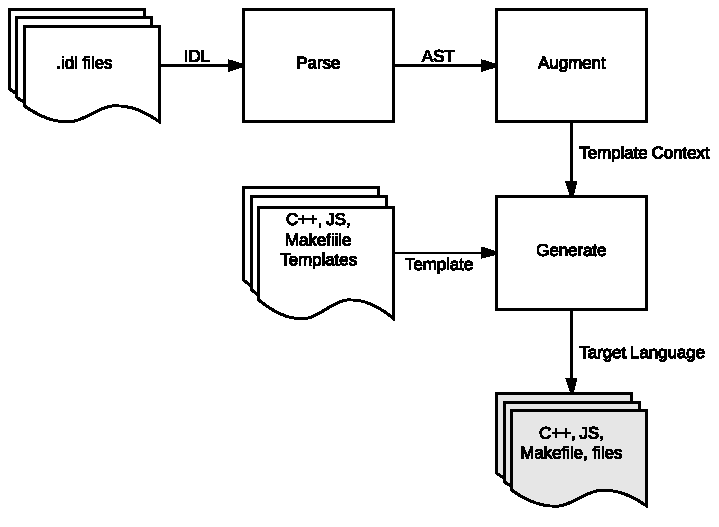
\includegraphics[width=0.9\textwidth]{generator.pdf} 
    \caption{Flow diagram showing the role of the generator}
    \label{fig:generator-diagram}
\end{figure}

We use the augmented AST as a \emph{context} to be passed to the template engine. We also add some helper functions on top of the template engine, to simplify the actual template. The template engine then uses the context to substitute the relevant strings into the correct places. For example, Listing \ref{code_template_context_eg} is a context that is used with the template shown in Listing \ref{code_template_eg} to generate the output shown in Listing \ref{code_template_output}. The rest of the code generator implementation is essentially augmenting the context to allow easy access for the template engine to generate all the files we needed.

Because the parser we used produces an AST in JavaScript, it made sense to have the generator in JavaScript too. This means we had to find a JavaScript template engine. There is more than a dozen template engine available to choose from, however, to simplify the templates and make them as human-readable as possible, we decided to limit our search only to templates with simple markup and logics. One template notation stood out, mustache\cite{mustache}. Mustache is an elegant, simple, templating language used across many languages. We decided to go with it because of its good documentation on its notation, its popularity, and its simplicity. However, several implementations of mustache existed. There was mustache.js\cite{mustachejs}, handlebars\cite{handlebarsjs}, and hogan\cite{hoganjs} by twitter. After considering each implementation, we found that they were very similar. We decided to choose hogan for its simplicity, speed, and extra features.

\lstset{language=JavaScript,caption={An example of a template context},label=code_template_context_eg}
\begin{code}
{
  timestamp: "Thu May 08 2014 21:38:16 GMT+0100 (BST)",
  moduleName: "Bullet",
  dictionaries: [{
    name: "XYZ",
    members: [
      { name: "x", STDTypeName: "float"},
      { name: "y", STDTypeName: "float"},
      { name: "z", STDTypeName: "float"}
    ]
  }]
}
\end{code}

\lstset{language=C,caption={An example of a template},label=code_template_eg}
\begin{code}
/* AUTOMATICALLY GENERATED ON {{timestamp}} */

#ifndef PPRPCGEN_{{moduleName}}_TYPES_H_
#define PPRPCGEN_{{moduleName}}_TYPES_H_

#include <string>
#include <vector>

namespace pprpcgen{
{{#dictionaries}}
typedef struct {
  {{#members}}
  {{^typeIsSequence}}{{STDTypeName}}{{/typeIsSequence}}
  {{#typeIsSequence}}std::vector<{{STDTypeName}}>{{/typeIsSequence}}
  {{name}};
  {{/members}}
} {{name}};

{{/dictionaries}}

}

#endif /* PPRPCGEN_{{moduleName}}_TYPES_H_ */

\end{code}

\lstset{language=C,caption={An example of the output of the generator},label=code_template_output}
\begin{code}
/* AUTOMATICALLY GENERATED ON Fri Jun 06 2014 20:11:41 GMT+0100 (BST) */

#ifndef PPRPCGEN_Bullet_TYPES_H_
#define PPRPCGEN_Bullet_TYPES_H_

#include <string>
#include <vector>

namespace pprpcgen{

typedef struct {
  float x;
  float y;
  float z;
} XYZ;

}

#endif /* PPRPCGEN_Bullet_TYPES_H_ */

\end{code}

% subsection code_generators_design (end)

% section generating_rpc_code (end)


